% define \title (only used by writelatex.com)
%\title{CSEC-793 Project Report_Blank}
%%%%%%%%%%%%%%%%%%%%%%%%%%%%%%%%%%%%%%%%%%%%%%%%%%%%%%%%%%%%%%%%%%%%%%
% LaTeX Template: Project Titlepage
%
% Source: http://www.howtotex.com
% Date: April 2011
% 
% This is a title page template which be used for articles & reports.
% 
% Feel free to distribute this example, but please keep the referral
% to howtotex.com
% 
%%%%%%%%%%%%%%%%%%%%%%%%%%%%%%%%%%%%%%%%%%%%%%%%%%%%%%%%%%%%%%%%%%%%%%
% How to use writeLaTeX: 
%
% You edit the source code here on the left, and the preview on the
% right shows you the result within a few seconds.
%
% Bookmark this page and share the URL with your co-authors. They can
% edit at the same time!
%
% You can upload figures, bibliographies, custom classes and
% styles using the files menu.
%
% If you're new to LaTeX, the wikibook is a great place to start:
% http://en.wikibooks.org/wiki/LaTeX
%
%%%%%%%%%%%%%%%%%%%%%%%%%%%%%%%%%%%%%%%%%%%%%%%%%%%%%%%%%%%%%%%%%%%%%%
%
% --------------------------------------------------------------------
% Preamble
% --------------------------------------------------------------------
\documentclass[ fontsize=11pt,twoside]{scrartcl}	% KOMA

\usepackage[letterpaper,pdftex]{geometry}	% A4paper margins
\setlength{\oddsidemargin}{5mm}			% Remove 'twosided' indentation
\setlength{\evensidemargin}{5mm}

\usepackage[english]{babel}
\usepackage[protrusion=true,expansion=true]{microtype}	
\usepackage{amsmath,amsfonts,amsthm,amssymb}
\usepackage{graphicx}
\usepackage{pseudocode}

\usepackage[latin1]{inputenc}
\usepackage{tikz}
\usetikzlibrary{shapes,arrows}


% --------------------------------------------------------------------
% Definitions (do not change this)
% --------------------------------------------------------------------
\newcommand{\HRule}[1]{\rule{\linewidth}{#1}} 	% Horizontal rule

\makeatletter							% Title
\def\printtitle{%						
    {\centering \@title\par}}
\makeatother									

\makeatletter							% Author
\def\printauthor{%					
    {\centering \Large \@author}}				
\makeatother							

% --------------------------------------------------------------------
% Metadata (Change this)
% --------------------------------------------------------------------
\title{	\Large \textsc{ TalkBox \\ 
															} 	% Subtitle
		 	\\[2.0cm]								% 2cm spacing
			\HRule{2pt} \\						% Upper rule
			\LARGE \textbf{\uppercase{User Manual}}	% Title
			\HRule{2pt} \\ [0.5cm]		% Lower rule + 0.5cm spacing
		%	\Large \today			% Todays date
		}

 \author{
		Group 15\\	
		EECS 2311\\	
         \\
		\\
        \texttt{} \\
}


\begin{document}
% ------------------------------------------------------------------------------
% Maketitle
% ------------------------------------------------------------------------------
\thispagestyle{empty}		% Remove page numbering on this page

\printtitle					% Print the title data as defined above
  	\vfill
\printauthor				% Print the author data as defined above
\newpage
% ------------------------------------------------------------------------------
% Begin document
% ------------------------------------------------------------------------------
\setcounter{page}{1}		% Set page numbering to begin on this page


%%%%%%%%%%%%%%%
%														%
% 			Main Contents            %
%														%
%%%%%%%%%%%%%%%

\section{Installation Instructions}

To install the TalkBox Configuration App, download the file "TalkBoxConfig.jar". 
\section{How to Get Started}
\medskip 
To get started, TalkBox configuration is composed of two modes allowing you to configure and playback the TalkBox device. You can toggle between these two modes by clicking the "Switch Modes" button in the corner of the bottom left panel of the configuration app. The mode selection that the configuration app is currently in will be displayed in text above the "Switch Modes". 

\medskip

1. Playback Mode

\medskip
\newline
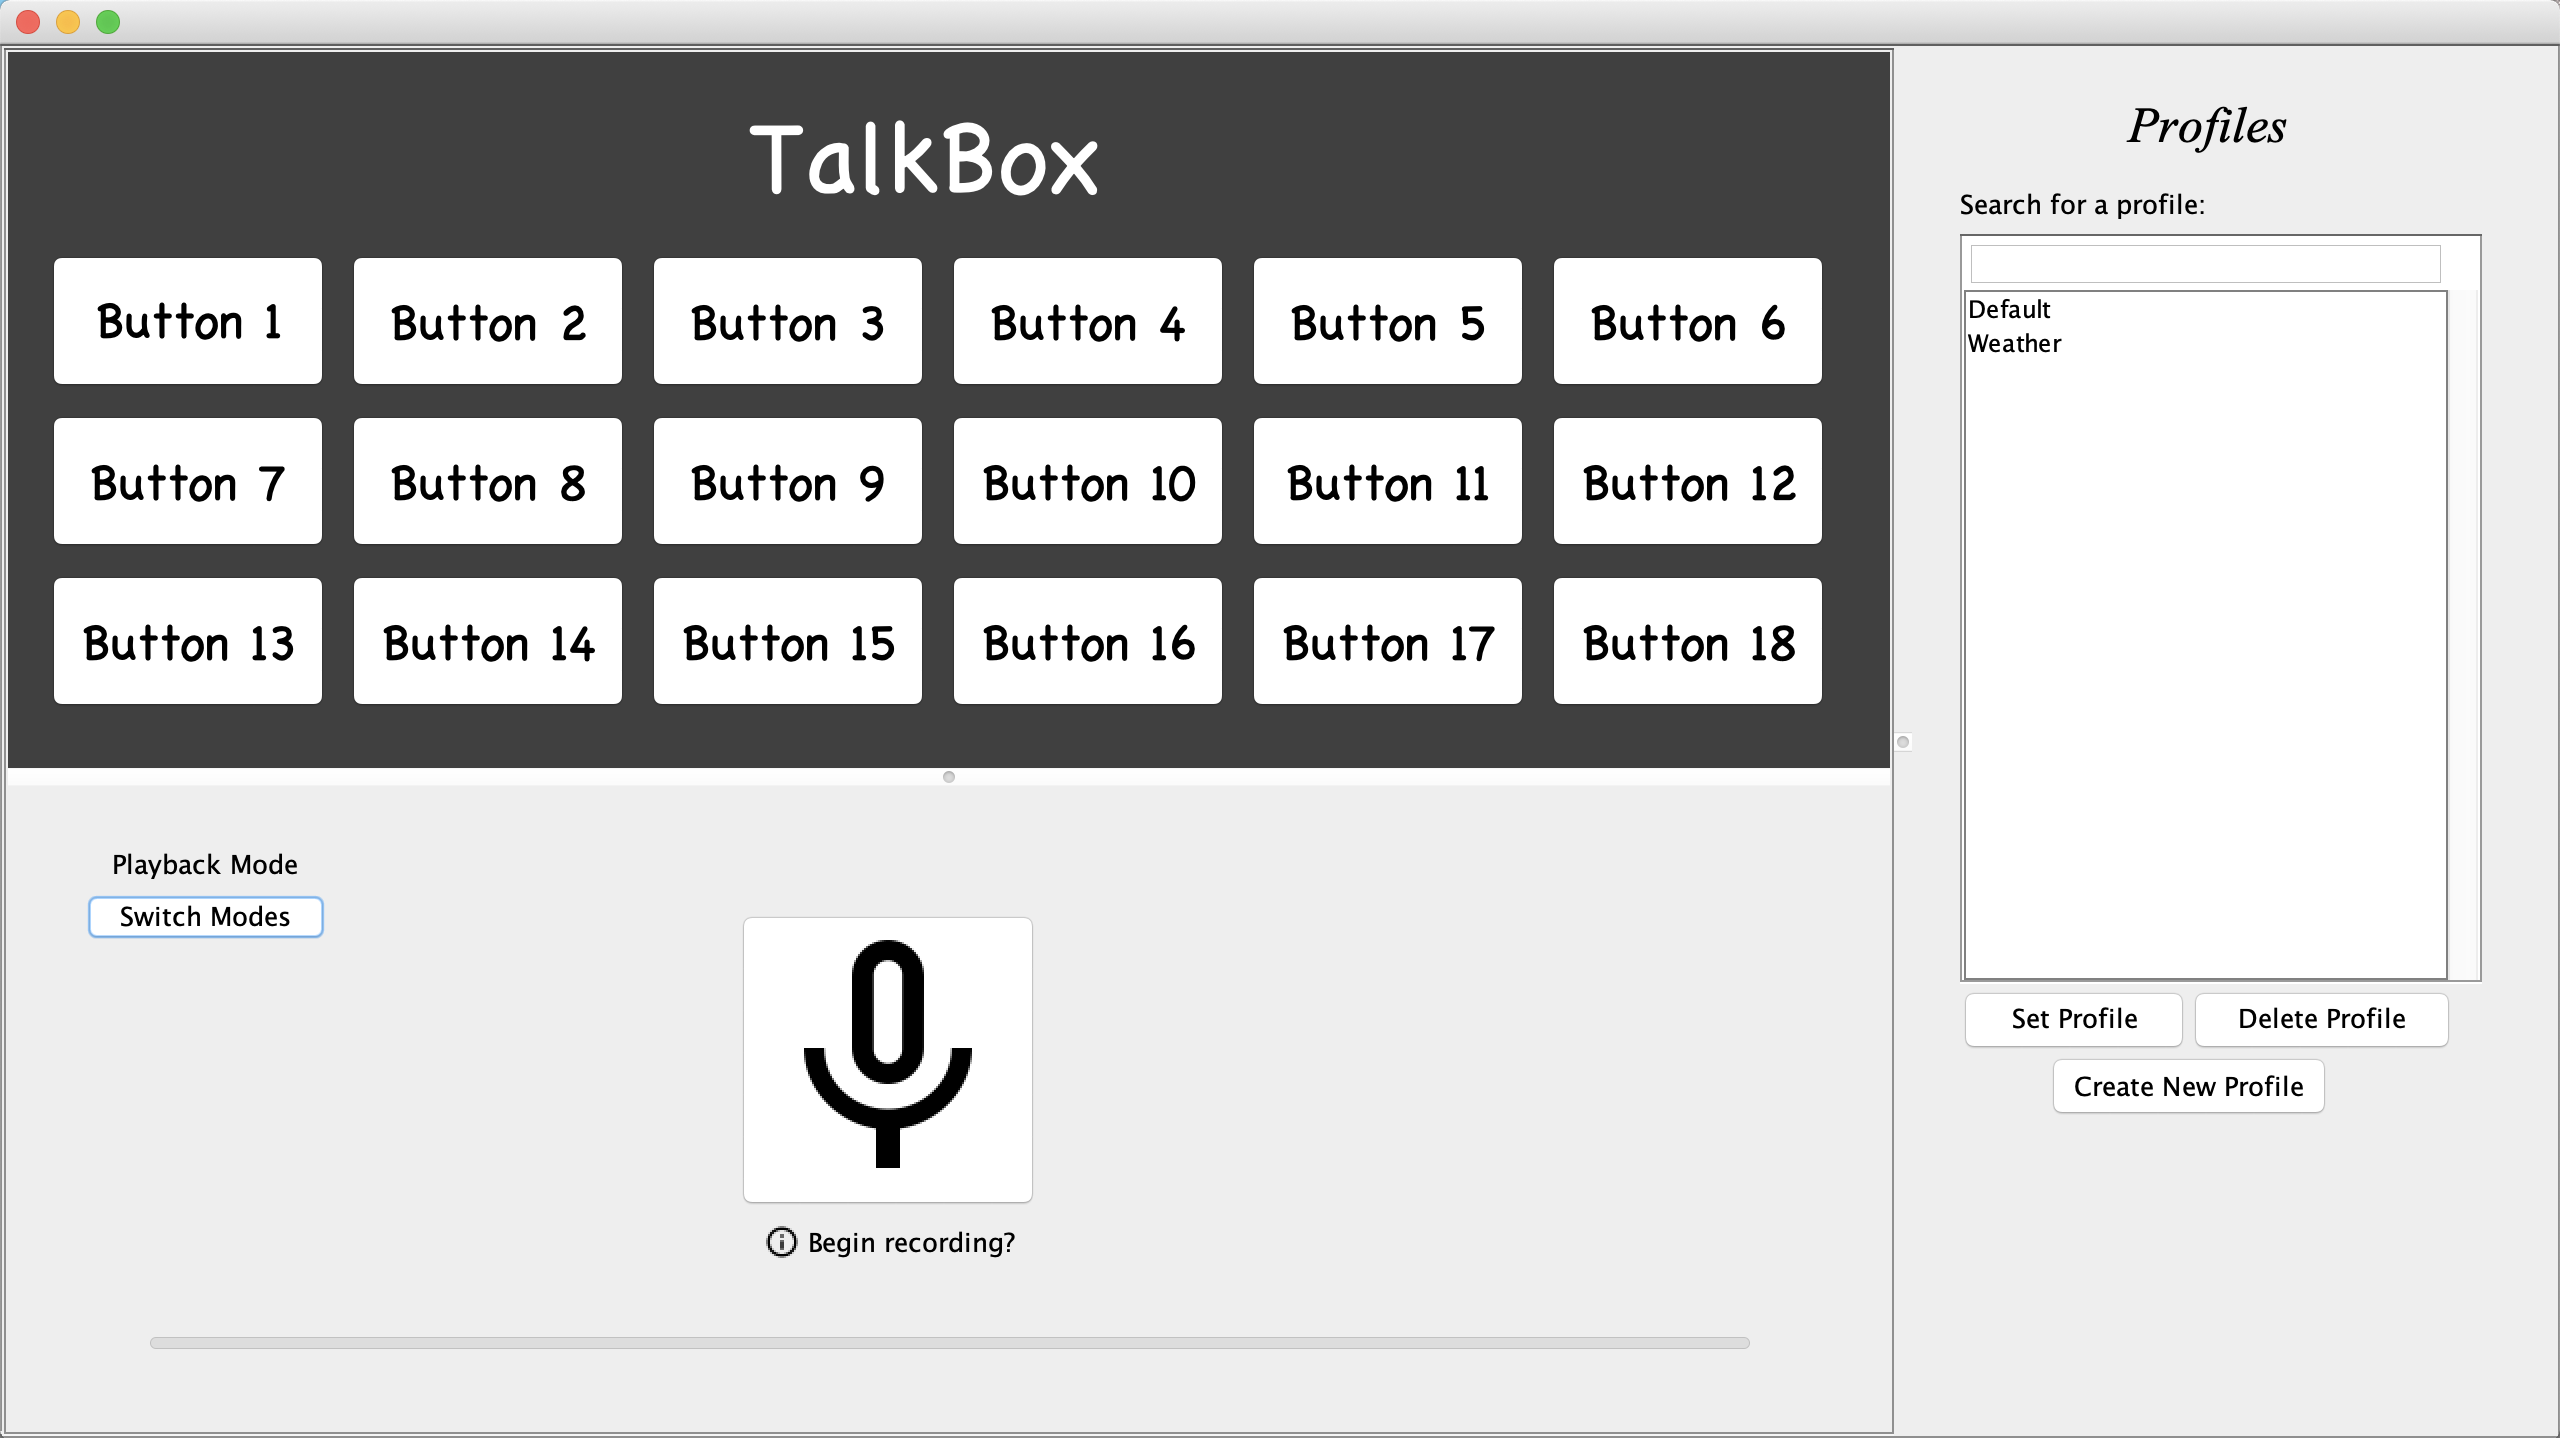
\includegraphics[width=\textwidth]{playback.png}
\medskip

In playback mode, the TalkBox device is simulated in the upper left panel. By clicking on the buttons, you can play back the recordings as the settings that the TalkBox device is currently set to. 
\medskip
\newpage

2. Edit Mode

\medskip

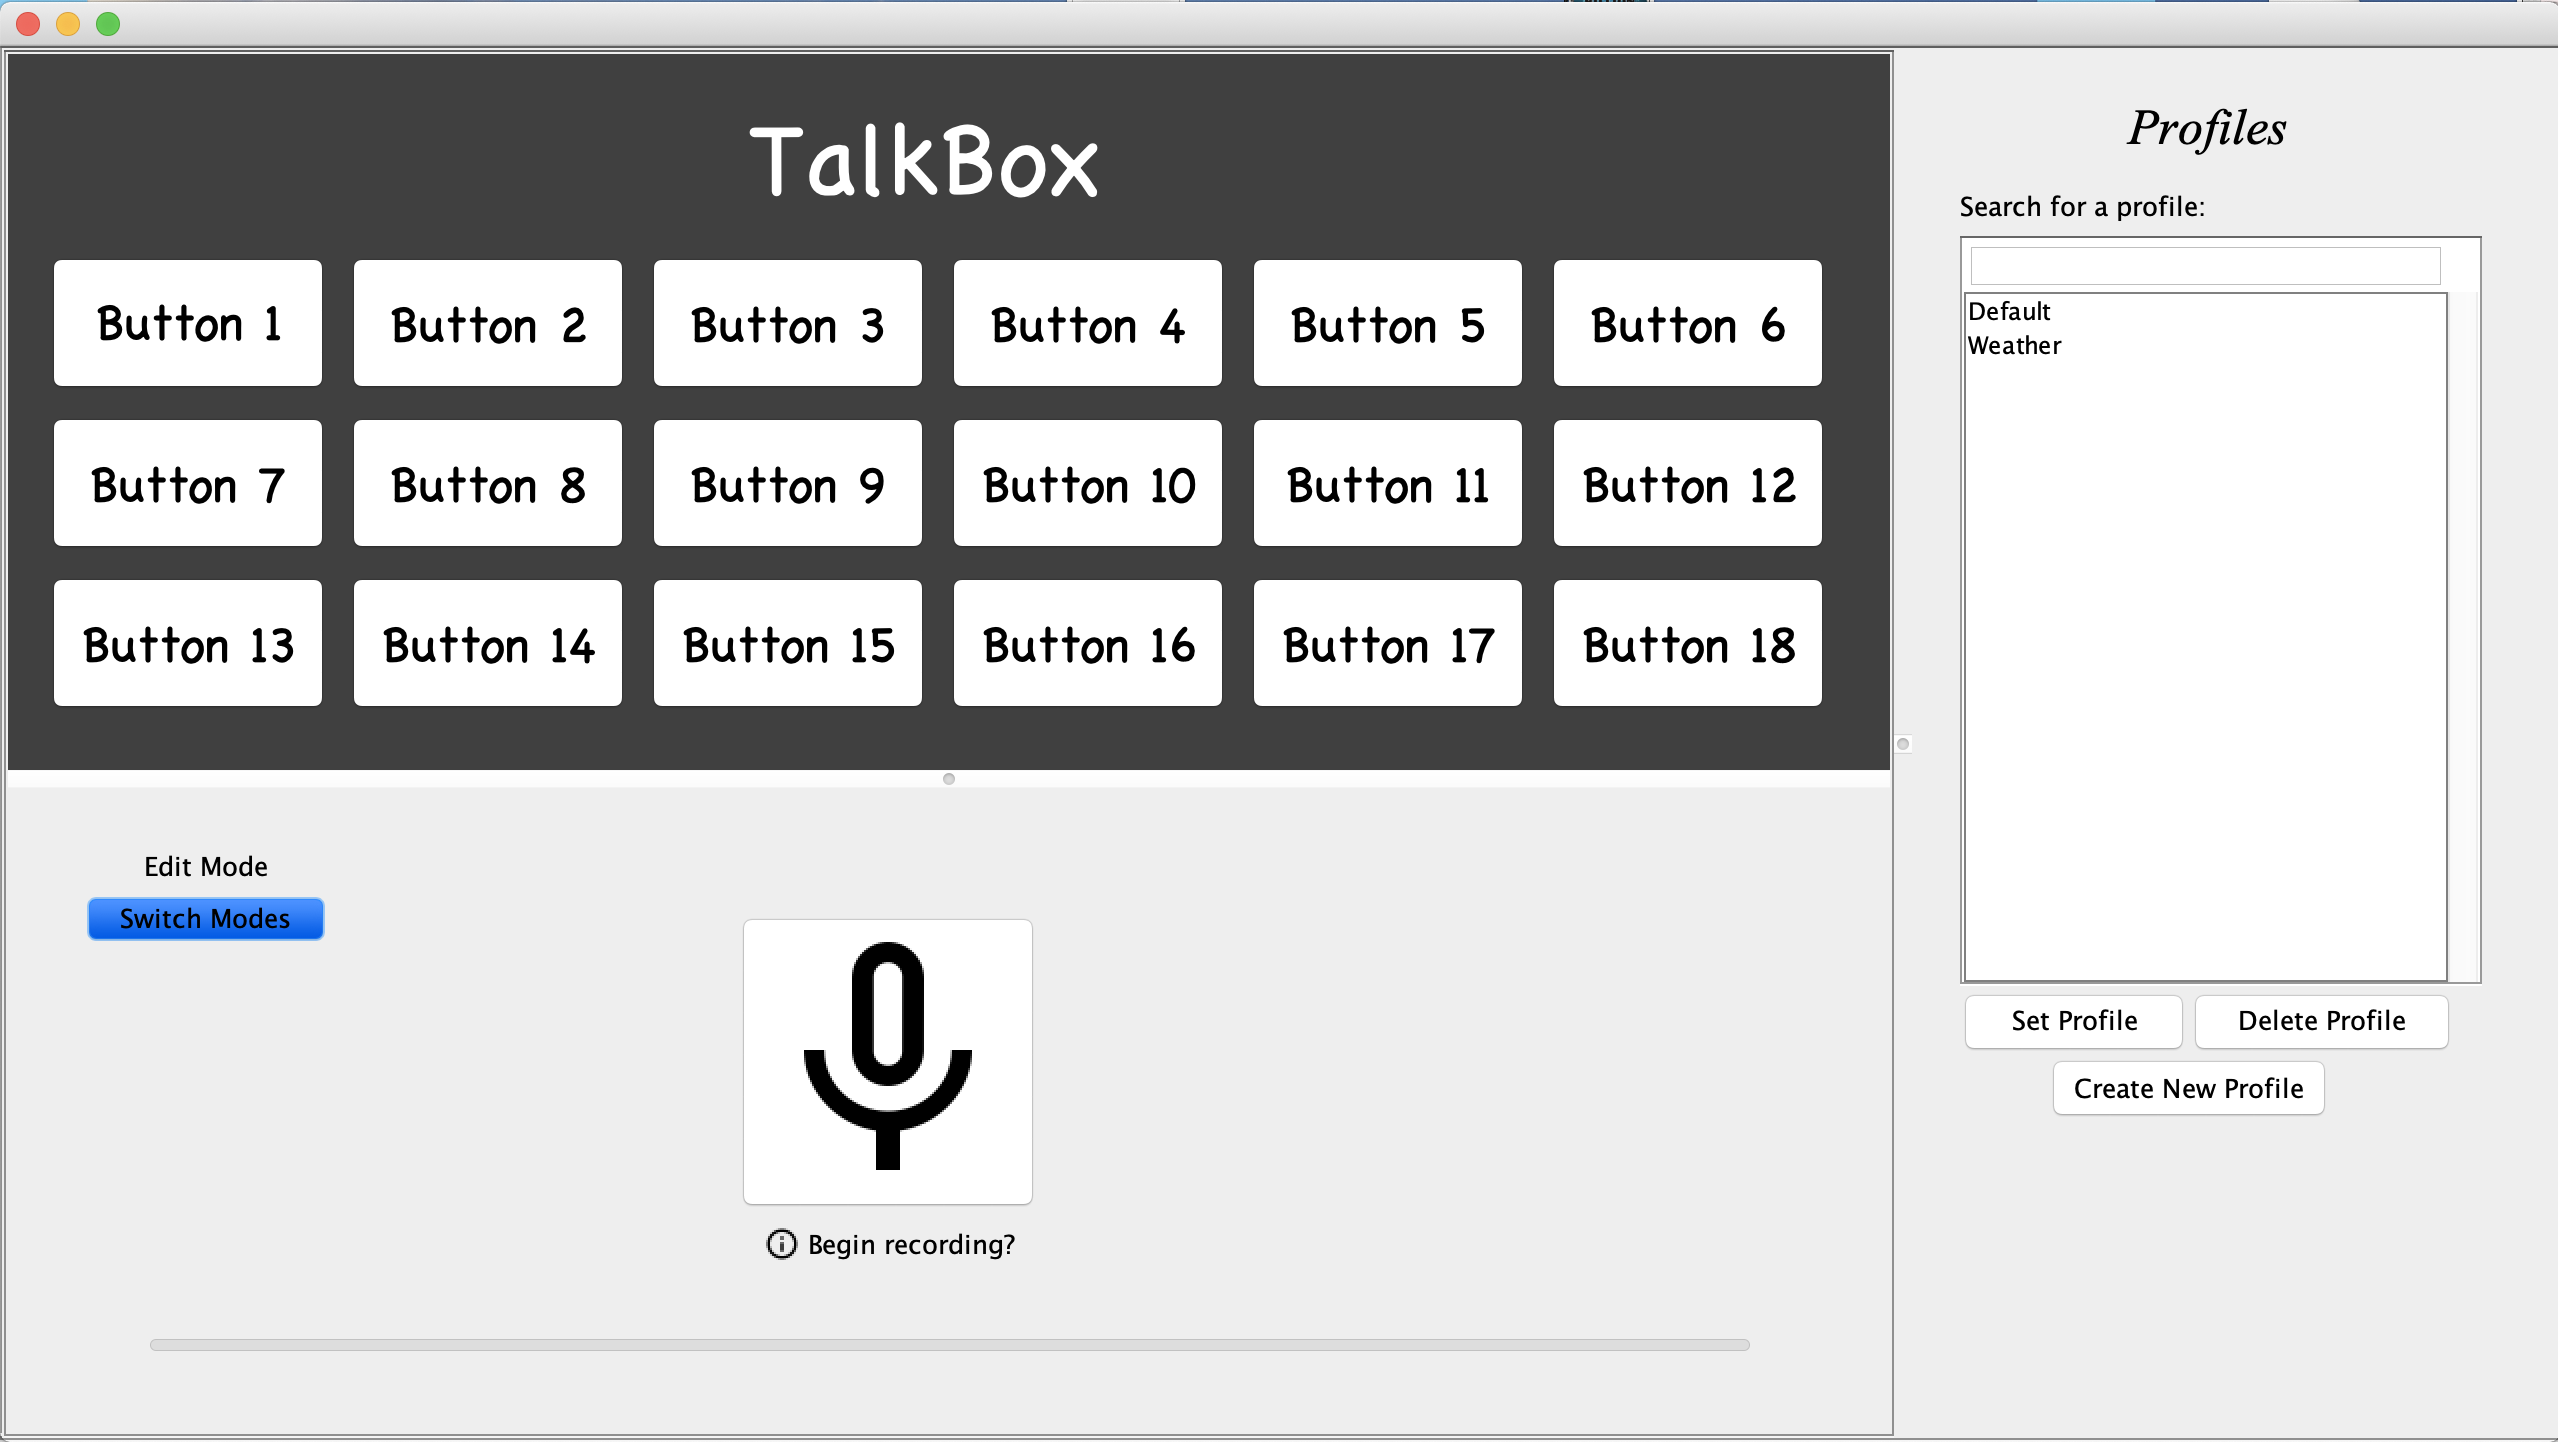
\includegraphics[width=\textwidth]{editmode.png}
\medskip

In edit mode, you can set up the configuration of the TalkBox device. In the profiles panel (on the right of the configuration app, you can load previously saved audio profiles, or create a new profile. When a profile is selected, its set of audio buttons are displayed in the simulation panel (top left of the configuration app). You can play back the audio files associated with buttons by clicking the buttons in the simulator. 

\newline
\medskip
To edit a specific button, click on the button you wish to edit. You can then click the "Record" button to record an new audio file, or select a previously saved audio file. To change the label of the button, select the button and input the new label name in the text box beside "Button Label:". The new label will now appear on the TalkBox simulator on the selected button. 







\section{Common Uses}

The TalkBox device is designed for users with a verbal impairment. The profiles loaded onto the TalkBox Device can be selected or adjusted based on user needs. Some common scenarios in which users may find the TalkBox device most useful are as follows. These common use scenarios are audio profiles and buttons that are pre-loaded onto the TalkBox device. 

\begin{enumerate}
\end{enumerate}
\begin{enumerate}
\item General purpose education: Yes, No, I understand, I don't understand, Can you explain more?, I would like assistance
\item Emotions: Happy, Sad, Excited, Confused, Anxious, Bored
\item Weather: Sunny, Rainy, Cloudy, Snowy, Icy, Hot, Warm, Chilly, Cold, Freezing, Windy
\item Hospital: Yes, No, I am in pain, I am okay, Help!
\item Restaurant: Menu, Water, Restroom, I would like to order something, Thank you, May I have the bill?
\end{enumerate}
\medskip

The TalkBox device is designed to be fully configurable based on user needs. Functions such as number of buttons or profiles on the TalkBox device can be determined by the user. It is recommended that these functions are determined based on consideration of the environment in which is it meant to be used. 
\newline 

For example, the "Hospital" profile listed above is limited to five  buttons, as a pressing situation such as a hospital visit may require a simple interface of only essential buttons. In comparison, profiles such as "Weather", most commonly used for daily journal-keeping or educational activities, can be more extensive in its descriptive level. 


%%\include{project_idea}
%%\include{project_implementation}
%%\include{project_testing}
%%\include{project_data_analysis}
%%\include{conclusion}
%%\include{acknowledgement}
%%\include{references}



% ------------------------------------------------------------------------------
% End document
% ------------------------------------------------------------------------------
\end{document}